\documentclass{article}
\title{Attention Is All You Need}
\author{Ashish Vaswani \and Noam Shazeer}
\begin{document}
\maketitle
\begin{abstract}
This compact fixture represents a public Transformer paper for parser integration tests.
\end{abstract}
\section{Introduction}
Sequence modeling motivates an architecture centered on attention operations.

This fixture paragraph exists to test stable paragraph identifiers and section linkage.
\section{Model Architecture}
\begin{figure}
\centering
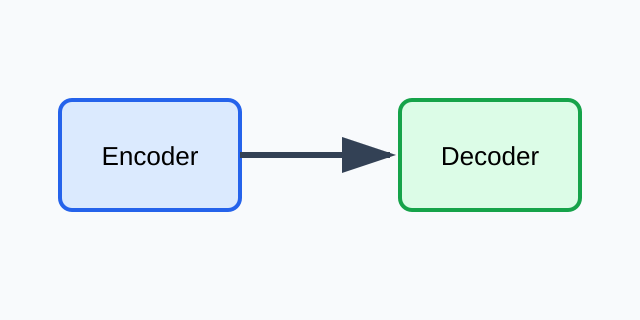
\includegraphics{figures/architecture}
\caption{Fixture diagram of an encoder and decoder flow.}
\label{fig:architecture}
\end{figure}
\begin{equation}
Attention(Q,K,V)=softmax(QK^T)V
\label{eq:attention}
\end{equation}
\subsection{Attention}
The attention block connects queries, keys, and values in this synthetic example.
\section{Experiments}
\begin{table}
\caption{Fixture evaluation results.}
\label{tab:results}
\begin{tabular}{lc}
System & Score \\
Fixture baseline & 10.0 \\
Fixture model & 11.0
\end{tabular}
\end{table}
The table contains invented values solely for software testing.
\end{document}

